\documentclass[12pt,fullpage,letterpaper]{article}

\newenvironment{proof}{\noindent{\bf Proof:}}{\qed\bigskip}

\newtheorem{theorem}{Theorem}
\newtheorem{corollary}{Corollary}
\newtheorem{lemma}{Lemma} 
\newtheorem{claim}{Claim}
\newtheorem{fact}{Fact}
\newtheorem{definition}{Definition}
\newtheorem{assumption}{Assumption}
\newtheorem{observation}{Observation}
\newtheorem{example}{Example}
\newcommand{\qed}{\rule{7pt}{7pt}}

\newcommand{\assignment}[4]{
\thispagestyle{plain} 
\newpage
\setcounter{page}{1}
\noindent
\begin{center}
\framebox{ \vbox{ \hbox to 6.28in
{\bf CS598: CXZ \hfill #1}
\vspace{4mm}
\hbox to 6.28in
{\hspace{2.5in}\large\mbox{Problem Set #2}}
\vspace{4mm}
\hbox to 6.28in
{{\it Handed Out: #3 \hfill Due: #4}}
}}
\end{center}
}


\newcommand{\handout}[3]{
\thispagestyle{plain} 
\newpage
\setcounter{page}{1}
\noindent
\begin{center}
\framebox{ \vbox{ \hbox to 6.28in
{\bf CS598: CXZ \hfill #1}
\vspace{4mm}
\hbox to 6.28in
{\hspace{2.5in}\large\mbox{#2}}
\vspace{4mm}
\hbox to 6.28in
{{\it Handed Out: #3 \hfill Name (NetID): \rule[-2pt]{4cm}{0.1pt} }}
}}
\end{center}
}


\newcommand{\assgsoln}[4]{
\thispagestyle{plain} 
\newpage
\setcounter{page}{1}
\noindent
\begin{center}
\framebox{ \vbox{ \hbox to 6.28in
{\bf CS598: CXZ \hfill #1}
\vspace{4mm}
\hbox to 6.28in
{\hspace{2.5in}\large\mbox{Problem Set #2 Solutions}}
\vspace{4mm}
\hbox to 6.28in
{{\it Handed Out: #3 \hfill Handed In: #4}}
}}
\end{center}
}


\newcommand{\solution}[4]{
\thispagestyle{plain} 
\newpage
\setcounter{page}{1}
\noindent
\begin{center}
\framebox{ \vbox{ \hbox to 6.28in
{\bf CS598: CXZ \hfill #4}
\vspace{4mm}
\hbox to 6.28in
{\hspace{2.5in}\large\mbox{Problem Set #3}}
\vspace{4mm}
\hbox to 6.28in
{#1 \hfill {\it Handed In: #2}}
}}
\end{center}
\markright{#1}
}


\newenvironment{algorithm}
{\begin{center}
\begin{tabular}{|l|}
\hline
\begin{minipage}{1in}
\begin{tabbing}
\quad\=\qquad\=\qquad\=\qquad\=\qquad\=\qquad\=\qquad\=\kill}
{\end{tabbing}
\end{minipage} \\
\hline
\end{tabular}
\end{center}}

\def\Comment#1{\textsf{\textsl{$\langle\!\langle$#1\/$\rangle\!\rangle$}}}



\oddsidemargin 0in
\evensidemargin 0in
\textwidth 6.5in
\topmargin -0.5in
\textheight 9.0in
\usepackage{amsmath}
\usepackage{graphicx}


\begin{document}

\solution{chen zhang, NetId: czhang49}{\today}{5}{Fall 2016}
% Fill in the above, for example, as follows:
% \solution{Joe Smith}{\today}{1}{Fall 2012}

\pagestyle{myheadings}  % Leave this command alone

\section{PLSA With and Without the Background Topic}

\subsection*{(a)}
When $\lambda = 0$, the second model is reduced to the first one. 

\subsection*{(b)}
\begin{align*}
p(w|D)= \dfrac{c(w,D)p(z=\text{background}|w)}{\sum_{w'\in D}c(w',D)p(z=\text{background}|w')}
\end{align*}

\subsection*{(c)}
If $\lambda$ is very large, the background model plays a big role. Then the topic words we found that have higher probability in the topic model will be those that have a small probability in the background model . On the other hand, If $\lambda$ is very small, then the topic words we found will be those that have a big probability in the documents with little consideration the background model.\\
To prove of refute this, we can use a given background language model, and set $\lambda$ to large values, use the EM algorithm for a collection of documents and see the resulting $p(w|\theta_i)$ for different $\theta_i$ and see if the top topic words are those that have small probability in the background model. Similarly we can set $\lambda$ to small values, use the EM algorithm for a collection of documents and see the resulting $p(w|\theta_i)$ for different $\theta_i$ and see if the topic words only have to do with the topic model. 

\section{Deriving the EM Algorithm for PLSA with a Background Topic}
\subsection*{(a)}
\begin{equation*}
n_{d,k} = \sum_{w \in d} c(w,d)q_y(y_{d,w}=1)q_{z|y}(z_{d,w}=k)
\end{equation*}
\begin{equation*}
n_{w,k} = \sum_{d \in D} c(w,d)q_y(y_{d,w}=1)q_{z|y}(z_{d,w}=k),
\end{equation*}
where $w$, $d$, $k$, $D$ represents a word, a document, a topic and the collection of documents. \\
Also we have the relation 
\begin{equation*}
q_y(y_{d,w}=1)q_{z|y}(z_{d,w}=k) = \dfrac{(1-\lambda)p(z_{d,w}=k|\pi_d^{(n)})p(w|\theta_k^{(n)})}{\lambda p(w|D)+(1-\lambda)\sum_{k'=1}^K p(z_{d,w}=k|\pi_d^{(n)})p(w|\theta_k^{(n)})}
\end{equation*}

\subsection*{(b)}
The update rule is :
\begin{equation*}
p(z=k|\pi_d^{(n+1)}) = \dfrac{n_{d,k}}{\sum_{k'=1}^K n_{d,k'}}
\end{equation*}
and
\begin{equation*}
p(w|\theta_k^{(n+1)}) = \dfrac{n_{w,k}}{\sum_{w'\in V} n_{w',k}}
\end{equation*}

\section{Implementing PLSA with a Background Topic}
\subsection*{(1)}
The code is as in the attachment czhang49-assignment5.zip.

\subsection*{(2)}
I predict the iteration V.S. log likelihood to be log-like increasing and converging to a specific value until convergence criteria is met. 

\subsection*{(3)}
I predict the iteration V.S. delta (relative difference in log likelihood) to be log-like decreasing and converging to a 0 until convergence criteria ($10^{-5}$) is met. 

\subsection*{(4)}
\begin{figure}[!ht]
  \centering
    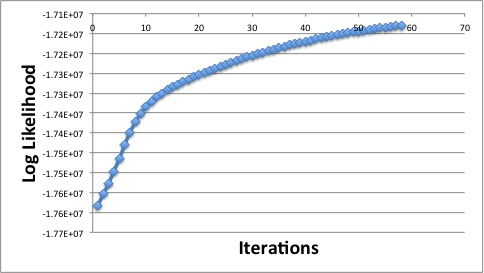
\includegraphics[width=\textwidth]{Lambda09Round1LogLikelihood.jpg}
      \caption{$\lambda = 0.9$, iteration V.S. log likelihood}
\end{figure}

\begin{figure}[!ht]
  \centering
    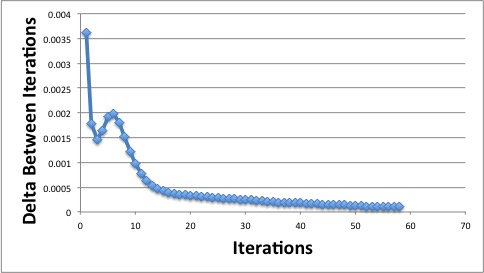
\includegraphics[width=\textwidth]{Lambda09Round1Delta.jpg}
      \caption{$\lambda = 0.9$, iteration V.S. delta (relative difference in log likelihood)}
\end{figure}
The figures are shown as in Figure 1 and Figure 2. \\
The shapes matched my prediction. \\
The log likelihood increase because essentially that's built in our EM formulation, and we want the likelihood function to increase. It converges when the maximum of expectation is achieved and the optimization problem is successfully solved. \\
The delta decreases because as the log likelihood converges, the difference between adjacent iterations become smaller and smaller. At the time where the EM algorithm converges and the optimization problem is solved, we could expect delta to be very close to zero.

\subsection*{(5)}
For $\lambda = 0.9$, the top 10 words for each topic are : \\
Topic 1: mining,
data,
patterns,
rules,
frequent,
rule,
pattern,
association,
itemsets,
database
\\
Topic 2:
image,
images,
retrieval,
video,
features,
similarity,
recognition,
semantic,
matching,
feature
\\
Topic 3:
cache,
data,
spatial,
memory,
queries,
caching,
prefetching,
caches,
access,
index
\\
Topic 4:
test,
testing,
loop,
regression,
tree,
suite,
communities,
tests,
cases,
signature
\\
Topic 5:
surface,
shape,
rendering,
mesh,
method,
texture,
motion,
point,
camera,
image
\\
Topic 6:
clustering,
web,
topic,
clusters,
cluster,
context,
text,
document,
documents,
aspect
\\
Topic 7:
query,
search,
queries,
ranking,
retrieval,
join,
feature,
results,
documents,
similarity
\\
Topic 8:
routing,
control,
placement,
access,
window,
exception,
coverage,
translation,
sentences,
role
\\
Topic 9:
type,
program,
programs,
analysis,
checking,
types,
flow,
safety,
analyses,
java
\\
Topic 10:
web,
code,
security,
compiler,
services,
pages,
business,
dynamic,
program,
workflow
\\
Topic 11:
service,
users,
traffic,
mobile,
privacy,
internet,
services,
group,
trust,
agents
\\
Topic 12:
xml,
schema,
query,
views,
view,
queries,
database,
schemas,
expressions,
facial
\\
Topic 13:
verification,
abstraction,
specification,
formal,
checking,
roles,
role,
agent,
specifications,
components
\\
Topic 14:
network,
sensor,
networks,
nodes,
wireless,
routing,
node,
protocol,
protocols,
sensors
\\
Topic 15:
software,
development,
engineering,
research,
design,
requirements,
evolution,
process,
tools,
usability
\\
Topic 16:
energy,
power,
consumption,
chip,
design,
processor,
performance,
embedded,
voltage,
hardware
\\
Topic 17:
language,
semantics,
logic,
transactions,
languages,
concurrency,
reasoning,
proof,
transaction,
fuzzy
\\
Topic 18:
performance,
memory,
parallel,
server,
scheduling,
processors,
disk,
execution,
storage,
file
\\
Topic 19:
graph,
graphs,
learning,
problem,
distance,
problems,
string,
labeled,
supervised,
classification
\\
Topic 20:
peer,
log,
pp,
distributed,
broadcast,
overlay,
peers,
nodes,
any,
bound
\\ \\ 
For $\lambda = 0.3$, the top 10 words for each topic are : \\
Topic 1:
of,
the,
and,
to,
language,
type,
in,
for,
we,
is
\\
Topic 2:
the,
of,
and,
in,
software,
to,
is,
this,
models,
for
\\
Topic 3:
and,
of,
in,
the,
to,
we,
for,
this,
applications,
these
\\
Topic 4:
the,
web,
to,
of,
and,
user,
users,
information,
in,
that
\\
Topic 5:
the,
to,
and,
of,
in,
security,
that,
system,
is,
we
\\
Topic 6:
the,
of,
and,
to,
we,
for,
is,
method,
in,
surface
\\
Topic 7:
the,
to,
of,
network,
and,
in,
networks,
nodes,
sensor,
we
\\
Topic 8:
the,
and,
of,
to,
in,
based,
this,
for,
systems,
is
\\
Topic 9:
the,
to,
of,
that,
is,
in,
execution,
code,
time,
and
\\
Topic 10:
the,
of,
is,
in,
that,
we,
algorithm,
for,
problem,
and
\\
Topic 11:
the,
of,
and,
for,
program,
to,
we,
in,
analysis,
programs
\\
Topic 12:
the,
of,
to,
in,
mining,
patterns,
test,
and,
is,
rules
\\
Topic 13:
the,
and,
of,
to,
for,
system,
we,
be,
model,
systems
\\
Topic 14:
data,
of,
the,
in,
and,
to,
is,
we,
on,
for
\\
Topic 15:
the,
and,
to,
of,
in,
routing,
that,
is,
this,
as
\\
Topic 16:
the,
and,
of,
to,
performance,
in,
on,
for,
memory,
that
\\
Topic 17:
the,
of,
is,
we,
to,
for,
that,
this,
on,
in
\\
Topic 18:
the,
and,
of,
to,
in,
we,
with,
motion,
that,
for
\\
Topic 19:
the,
query,
of,
queries,
to,
and,
in,
we,
data,
for
\\
Topic 20:
the,
of,
and,
to,
in,
is,
on,
we,
based,
for
\\ \\
For large $\lambda$, the words are descriptive topic words. For small $\lambda$, the words are not descriptive, mostly stop words. \\
This is expected, because when $\lambda$ is large, the background model plays a big role. In this case, increasing the probability of words in the topic model which already have large probability in the background model does not increase the overall likelihood very much. On the contrary, increasing the the probability of words in the topic model which have small probability in the background model will increase the overall likelihood very much. So in this case we will see descriptive topic words having higher probability in the topic model.  \\
When $\lambda$ is small, the background model is not considered much, so the words with higher probability in the documents will have higher probability in the topic model. These words are often stop words. \\
So if someone wants to find very descriptive topic words, I recommend using a large value $\lambda$. $\lambda>0.9$ seems to work well for the current setting. 

\subsection*{(6)}
We can have a repository of stop words (or words that we think will have very little implication on the document topics), and filter out those words before we run the algorithm to find the topic words. 

\subsection*{(7)}

\begin{figure}[!ht]
  \centering
    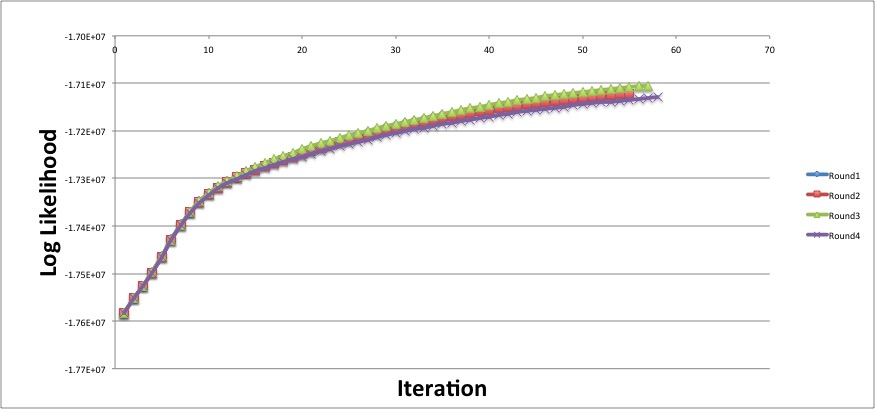
\includegraphics[width=\textwidth]{4RoundsLogLikelihood.jpg}
      \caption{$\lambda = 0.9$, iteration V.S. Log Likelihood for four different runs with $K=20, \lambda=0.9$.}
\end{figure}


The figure is shown in as Figure 3. \\
The four runs reach pretty much the same log likelihood value. This is true in general. Because for the same number of topics and same value of $\lambda$, the maximum of the expectations is the same due in the EM formulation. This is due to the fact that the EM algorithm is essentially solving for the solution to an optimization problem. Maybe for some problems, there are multiple local maximum which could result in different final log likelihood. But for most of the problems we are interested in, with fixed value of $K$ and $\lambda$, the problem is concave and has only one maximum value.  \\
I suggest using as small value of delta criteria as possible (relative difference in log likelihood in adjacent runs), in order to achieve higher log likelihood. 

\end{document}

